\documentclass[12pt]{article}
\usepackage[english]{babel}
\usepackage[utf8]{inputenc}
\usepackage{color}
\usepackage[a4paper,lmargin={2cm},rmargin={2cm}, tmargin={2cm},bmargin = {2cm}]{geometry}
\usepackage{amssymb}
\usepackage{amsmath}
\usepackage{mathtools}
\usepackage{graphicx}
\usepackage{cite}
\usepackage{wallpaper}
\usepackage{amstext}
\usepackage{blindtext}
\usepackage{multicol}
\usepackage[singlespacing]{setspace}
\usepackage{tabulary}
\usepackage{tabularx}
\usepackage[T1]{fontenc}
\usepackage{float}
\usepackage{csquotes}
\usepackage{todonotes}
\usepackage{gensymb}
\usepackage{pgfgantt}
\usepackage{pdflscape}

\usepackage{placeins}
\usepackage{afterpage}

\renewcommand{\labelitemi}{$\bullet$}
\renewcommand{\labelitemii}{$\cdot$}
\renewcommand{\labelitemiii}{$\circ$}
\renewcommand{\labelitemiv}{$\ast$}

\usepackage{caption}
\usepackage{framed}
\definecolor{shadecolor}{rgb}{0.6,0.6,0.61}

%\bibliographystyle{alphadin}
\bibliographystyle{IEEEtran}

\begin{document}
%\hyphenation{Ver-schlüsselungs-verfahren}

\begin{titlepage}
\ThisCenterWallPaper{1.0}{h-logo-background}	

%  \HoleMask

%  \hspace{-3cm}
  \begin{minipage}[t]{10cm}
  %\vspace{2cm}
  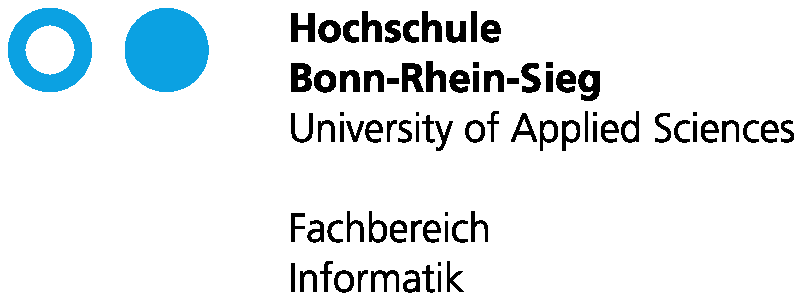
\includegraphics[width=10cm]{h-logo-full-font-embed}\\
  \end{minipage}
  \vspace{2.5cm}

	\begin{center}

    \vspace{0.8cm}

    \vspace{3cm}
    \begin{Huge}
    \textbf{Exposé}\end{Huge}\\
    \vspace{0.8cm}
  	\begin{huge}
  	\textbf{Einbindung von Constraints in eine divergente Optimierungsmethode am Beispiel der Surrogat-assistierten Illumination}
  	\end{huge}
  	 \vspace{0.6cm} \\
  	  	  \begin{large}von
  	  \end{large}
  	  \\ \begin{LARGE}
  	   \vspace{0.6cm}
  	  {Jan Kruska}\\
  	  9028385\\
  	  \vspace{0.8cm}
  	 
  	\end{LARGE}
  	
    \vspace{3.0cm}
			\end{center}
	\begin{large}
%	\begin{flalign}
%	\hspace{4.5cm} 
	%\text{Referee and Tutor:} \hspace{1.2cm}		&\text{Prof. Dr. Alexander Asteroth}& % \notag\\&31.12.2016  \notag
%\end{flalign} 

\begin{table}[h!]
\begin{tabularx}{\textwidth}{l@{\hspace{2.0cm}}X}

Betreut durch: & Prof. Dr. Alexander Asteroth\\
und: &  Alexander Hagg, M.Sc.\\



\end{tabularx}
\end{table}  
  
\end{large}
%  \vspace{0.5cm}
%  \vfill
\end{titlepage}


\pagenumbering{arabic}
\tableofcontents
\newpage{}


\section{Einleitung}

Die Domäne der Aerodynamik stellt durch ihre Komplexität sowohl für Mensch als auch Computer eine große Herausforderung dar.
Die physikalischen Gesetze, denen diese folgt, sind zwar bekannt, deren Zusammenspiel allerdings so stark ineinander verwoben, das beim Design aerodynamischer Körper oft auf Faustregeln zurückgefallen werden muss.

Evolutionäre Taktiken haben sich in der Vergangenheit als mächtige Heuristik zur Optimierung komplexer Problemräume bewiesen \cite{Vikhar.2016}.

Genetische Algorithmen sind eine effektive Methode um kreative Lösungen für komplexe Probleme zu generieren.
Allerdings haben evolutionäre Algorithmen ohne Zusatzmechanismen die Tendenz, dass gefundene Lösungen im Verlauf der Algorithmen zu einer Lösungsklasse konvergieren \cite{Shir.2012}.
Dies führt zu zwei Hauptproblemen.
Erstens neigen solche Algorithmen dadurch dazu in lokalen Optima "stecken" zu bleiben, da das Verlassen eines lokalen Optimums immer mit einer Fitnesseinbuße verbunden ist.
Zweitens produzieren solche Algorithmen nur eine Lösung.
Sollten mehrere gute Lösungen existieren, deren Fitness sich nur gering unterscheidet, wird trotzdem die Lösung, die um einen Bruchteil besser ist bestehen bleiben.
Häufig kann es allerdings sinnvoll sein auch diese Lösungen zu erhalten, da ein menschlicher Beobachter dadurch mehr Wissen erhalten kann welche Eigenschaften, für gute Lösungen sorgen, wenn sie beispielsweise häufig vorkommen, oder ob bestimmte Eigenschaften nur in Kombination gute Lösungen ergeben.
Dieses Wissen, was aus der Vielzahl an guten Lösungen gezogen werden kann, kann dabei helfen das Problem besser zu verstehen, was eine sehr wertvolle Eigenschaft ist.

Es wurden verschiedene Diversitätsansätze vorgeschlagen, die sich grundsätzlich in genotypische und phänotypische Diversitätsansätze unterscheiden lassen.
Ansätze wie Niching, gewährleisten genotypische Diversität durch die Ermittlung der genetischen Ähnlichkeit zweier Individuen.
Das hat den Vorteil, dass der Genotyp eines Individuums typischerweise ein Vektor ist, und eine Vielzahl von Ähnlichkeitsmetriken für Vektoren existiert.
Andere Ansätze verfolgen das Ziel phänotypischer, sprich funktionaler, Diversität.
Dies hat den Grund, dass die Funktion eines Individuums und nicht die Encodierung das eigentliche Optimierungsziel ist,
und in komplexen Problemdomänen sich genetisch sehr verschiedene Individuen trotzdem funktional ähneln können.
Um phänotypische Diversität zu gewährleisten wird allerdings eine phänotypische Ähnlichkeitsmetrik benötigt, die sehr domänenspezifisch ist.
Diese Ansätze werden allgemein unter dem Begriff der Quality-Diversity-Algorithmen zusammengefasst.
Diese liefern typischerweise eine Vielzahl möglicher Lösungen, durch die das Problem und Zusammenhänge zwischen Lösungseigenschaften und Lösungsqualität besser verstanden werden kann.



\section{Problembeschreibung}

Es ist bei allen Optimierungsmethoden, und damit auch bei genetischen Algorithmen im Speziellen, häufig der Fall, dass neben dem Primären Optimierungsziel, hier die Aerodynamik eines Bauteils, weitere Nebenbedingungen, auch Constraints genannt, eingehalten werden müssen.
Solche Constraints können durch sekundäre Anforderungen an Bauteile entstehen, die erfüllt sein müssen, oder erfüllt sein sollten.
Constraints, die erfüllt sein müssen, stellen absolute Ausschlusskriterien dar, und können im Verfahren durch einen Hard Constraint ermöglicht werden, durch den solche Lösungen, die den Constraint nicht erfüllen, gar nicht zugelassen werden.
Das führt dazu, dass nur Lösungen erzeugt werden können, die den Constraint auch erfüllen, hat allerdings den Nachteil, dass Diversität eingeschränkt werden kann und Optimierungsverfahren keine oder nur wenige sinnvollen Lösungen generieren, wenn der Constraint schwer zu erfüllen ist.
Stattdessen kann ein Soft Constraint genutzt werden, bei der Lösungen, die diesen nicht erfüllen mit einem Strafwert versehen werden.
Dies hat den Vorteil, dass auch Lösungen die den Constraint nicht erfüllen als Trittbrett zu solchen, die ihn erfüllen, genutzt werden können.
Dadurch besteht allerdings die Möglichkeit, dass ein Verfahren Lösungen produziert die den Constraint nicht erfüllen.
Auch ist die Frage wie ein Soft Constraint in ein Verfahren eingebaut und gewichtet wird komplizierter, ein zu schwach gewichteter Constraint kann dazu führen, dass das Verfahren diesen einfach ignoriert, was nicht Ziel der Optimierung war.
Die Frage ob ein Hard- oder Soft Constraint sinnvoller ist hängt stark von der Problemdomäne ab.

\subsection{Radkastendomäne}
\missingfigure{Radkästen}

Die erste Problemdomäne befasst sich mit der Verformung der Radkästen eines Velomobils. 
In Abb. \ref{fig:wheelcase} ist das das Velomobil mit eingezeichneten Radkästen zu sehen.
Es sollen beide Radkästen des Velomobils verformt werden, der Einfachheit halber kann diese Verformung aufgrund der Symmetrie des Velomobils symmetrisch zur xz-Ebene
\footnote{\label{foot:coords} Unter Annahme, dass die x-Achse die horizontale Vor/Rückachse, die y-Achse die horizontale Links/Rechtsachse und die z-Achse die Vertikalachse ist} stattfinden, sodass eine Deformation die Anweisungen für beide Radkästen enthält.
Die momentanen Radkästen schränken den vollen Lenkausschlag der Räder des Velomobils ein.
Es ist das Ziel Lösungen zu ermitteln, die den vollen Lenkausschlag ermöglichen.
Dadurch das die bestehenden Radkästen den Constraint nicht erfüllen und damit die Suche nach aerodynamisch sinnvollen Lösungen, das Problem darstellt bietet sich ein Hard Constraint nicht an.
Ein Soft Constraint, der Lösungen zulässt die den Constraint nicht erfüllen, scheint in einer solchen explorativen Suche nach Lösungen die den Constraint erfüllen weitaus sinnvoller.
Dadurch eröffnet sich allerdings die Frage wie dieser berechnet werden kann, vor allem in Anbetracht der Tatsache, dass dieser sehr häufig berechnet werden und damit effizient berechenbar sein muss.

                      
\subsection{E-Roller-Domäne}
\missingfigure{E-Roller-Abdeckung}

Die zweite optionale Problemdomäne ist ein E-Roller an dessen Unterseite ein Bauteil vor dem Hinterrad verformt werden soll.
In Abb. \ref{fig:escooter} ist der E-Roller zu sehen. Das zu verformende Bauteil ist rot hervorgehoben.
Auch für den E-Roller kann die Verformung symmetrisch zur xz-Ebene \footnote{Siehe Fußnote \ref{foot:coords}} erfolgen um den Suchraum zu verkleinern.
Auch für den E-Roller müssen Constraints eingehalten werden. 
So darf das Bauteil nicht beliebig weit nach unten verformt werden, da dies zu Kollisionen mit der Fahrbahn führen würde.
Gleichzeitig darf das verformte Bauteil bestehende Elemente des E-Rollers nicht schneiden.
Anders als in der Radkastendomäne erfüllt das Basisbauteil diese Constraints schon, Ziel ist also nur die Verbesserung des Luftwiederstands ohne dabei die Constraints zu verletzen.
 
\section{Literatur}

\subsection{MAP-Elites}
\label{sub:mapElites}
MAP-Elites \cite{Mouret.4202015} ist ein genetischer Algorithmus mit Diversitätsmanagement.
Ein wichtiger Aspekt von MAP-Elites ist, dass Diversität des Phänotyps gewährleistet wird.
Das bedeutet, dass die Morphologie bzw. Funktionalität einer konkreten ausgedrückten Lösung, wie beispielsweise Volumen oder Krümmung eines Bauteils, betrachtet wird, statt einer Distanz im Genotyp.
Dazu wird der Lösungsraum entlang beliebig vieler Feature-Dimensionen, d.h. Merkmalen der Lösungen, aufgeteilt.
Diese Feature-Dimensionen werden, mithilfe eines Minimums, Maximums und einer Anzahl an Schritten, diskretisiert wodurch der Lösungsraum in Zellen eingeteilt wird.
Diese Aufteilung wird häufig auch Karte genannt.
Jede dieser Zellen stellt dabei eine Kombination der Eigenschaften dar.
Zu jeden Zeitpunkt kann jeder dieser Zellen nur eine oder keine Lösung enthalten
\footnote{Eine Zelle kann nur keine Lösung enthalten wenn sie noch nicht befüllt wurde. Zellen können nicht entleert werden}.
In jeder Genration werden aus den momentan in der Karten enthaltenen Lösung Kinder erzeugt.
Jedes dieser Kinder wird bezüglich dessen Fitness evaluiert und nach den gewählten Features kategorisiert.
Damit wird diesem eine Zelle zugewiesen, in der lokale Konkurrenz stattfindet.
Ist die zugewiesene Zelle leer befüllt das Kind die Zelle, befindet sich bereits ein Individuum in der Zelle werden stattdessen die Fitnesswerte der beiden verglichen und das Individuum mit der höheren Fitness wird der Zelle zugewiesen.
Neben einer Vielzahl von Lösungen kann diese Karte auch dabei helfen die Problemdomäne besser zu verstehen, indem Zusammenhänge zwischen den Features, nach denen klassifiziert wurde und der Qualität der Lösungen, aufgedeckt werden.

\subsection{Surrogat-Modell}
\label{sub:surrogate}
Für die Selektion von Individuen innerhalb eines genetischen Algorithmus wird die Lösungsqualität dieser Individuen, typischerweise Fitness genannt, benötigt.
Außerdem findet die Auswertung der Fitnessfunktion innerhalb des genetischen Algorithmus sehr häufig statt.
Dies stellt bei relativ einfachen Fitnessfunktionen keine große Einschränkung dar, auf Problemdomänen in denen die Auswertung der Fitness eines Individuums allerdings komplexer und dadurch zeitaufwändiger wird, kann dies die Anwendbarkeit einfacher genetischer Algorithmen einschränken.

Aerodynamische Probleme, für die zeitaufwendige Simulationen nötig sind, gehören ohne Zweifel zu der Klasse von Problemen für die die Anzahl der benötigten Funktionsauswertungen zu groß sind, als das der Algorithmus in vertretbarer Laufzeit abschließen kann.
Um genetische Taktiken auf eine solche Problemdomäne anzuwenden, wird eine Möglichkeit benötigt die benötigten Funktionsauswertungen erheblich zu reduzieren.
Eine solche Möglichkeit ist ein Surrogatmodell \cite{Jin.2011}\cite{Preen.2016}, eine Machine-Learning Modell, welches aufgrund echter Simulationsauswertungen trainiert wird um deren Ergebnis annähernd vorherzusagen.
Eine Auswertung des Modells erfordert dabei nur einen winzigen Bruchteil des Aufwands der für eine Simulation nötig wäre.
Theoretisch sind verschiedenste Machine-Learning Verfahren für das Surrogatmodell denkbar, Gaußprozesse \cite{Rasmussen.2008} bieten sich durch die Eigenschaft an, dass sie neben einer Vorhersage auch immer ihre eigene Unsicherheit Liefern, und entsprechend Bereiche zeigen können in denen große Unsicherheit herrscht, oder anders ausgedrückt in denen der Gaußprozess wenig weiß.
Der Nachteil der hohen Speicher- und Berechnungskomplexität von Gaußprozessen ist durch die Limitierung auf eine geringe Anzahl an Simulationen, und damit der Limitierung auf einen kleinen Trainingsdatensatz vernachlässigbar.

\subsection{Freiformdeformation}

Freiformdeformation\cite{Sederberg.1986} ist ein Verfahren zu Deformation von geometrischen Objekten.
Es ist in der Lage 3D-Meshes anhand bestimmter Parameter zu verformen.
Dazu wird eine Box aus Kontrollpunkten erzeugt.
Jeder dieser Kontrollpunkte kann dann anhand von Verformungsparametern verschoben werden, wodurch für alle Punkte innerhalb der FFD-Box eine Verschiebung berechnet wird, die von der relativen Position des Punkt zum Kontrollpunkt abhängt.
Dadurch kann eine Deformation auf eine überschaubare Anzahl an Deformationsparametern reduziert werden.
Außerdem kann eine Deformation auf einige bestimmte Punkte und/oder Richtungen
\footnote{Deformation in x,y,z finden jeweils separat statt} 
beschränkt werden um die Komplexität weiter zu reduzieren.
Dadurch das nur die Punkte des Meshes ihre Position ändern, hat das Verfahren, den Vorteil das die Dreiecke erhalten bleiben und somit beispielsweise das Entstehen von Löchern bei korrekter Anwendung praktisch ausgeschlossen ist.

\subsection{SAIL}

SAIL (Surrogate-Assisted Illumination) vereint die in \ref{sub:mapElites} und \ref{sub:surrogate} beschriebenen Ansätze.
In \cite{Gaier.6152018} wurde gezeigt, dass dieser Ansatz erfolgreich auf 2D und 3D aerodynamische Domänen angewandt werden kann.
Es wurden Freiform-Deformationen auf 3D-Bauteile angewandt, welche dann wiederum bezüglich ihrer aerodynamischen Eigenschaften ausgewertet wurden um ein Surrogat-Modell zu trainieren.

\section{Ansatz}

Der bestehende Ansatz von SAIL ist in der Lage dreidimensionale Objekte zu verformen, ein Surrogat-Modell auf Basis von OpenFOAM \cite{OpenCFD.} Strömungssimulationen zu trainieren und mit diesem Surrogatmodell MAP-Elites anzuwenden. 
In diesen Ansatz sollen Constraints eingebunden werden.
Eine sinnvolle Definition der Constraints ist dabei die Hauptaufgabe.
In jeder Domäne muss eine Abwägung zwischen der Nutzung von Hard- oder Soft Constraints stattfinden.
Diese Constraints sollen dann entsprechend eingebunden werden, um zu untersuchen wie sich unterschiedliche Constraints auf das Verfahren auswirken.



\subsection{Velomobil}
Aufgrund der Tatsache, dass im momentanen Zustand der Constraint noch nicht erfüllt ist ist ein harter Constraint, der solche Lösungen, die ihn nicht erfüllen nicht zulässt nur schwer umzusetzen, da am Anfang des Prozesses keine bekannte valide Lösung existiert.
Weiche Constraints lassen es zu, dass Lösungen existieren die den Constraint erfüllen, in der Hoffnung, dass diese als Trittbrett zu Lösungen, die ihn erfüllen genutzt werden können.
In einer vorigen Arbeit wurde ein solcher Ansatz verfolgt, allerdings wurde hier ein konstanter Strafwert addiert, wenn der Constraint verletzt war.
Man könnte einen variablen Strafwert einfügen, der abhängig davon wie stark der Constraint verletzt wird größer oder kleiner ist, um dem Algorithmus einen Gradienten zu validen Lösungen zu geben.
Als Fehlermaß für die Qualität der am Ende produzierten Lösungen kann der Anteil am maximalen Radausschlag der erreicht wurde genutzt werden.
\todo[inline]{konkrete formel, schnitt kugel radkasten? oder schnitt kreise in  bspw. 1$\degree$ azimuth}

Um Verformungen an den Ränder der Radkästen, und die dadurch resultierenden scharfen Kanten zu vermeiden, sollten primär innere Punkte als Deformationspunkte gewählt werden.

Als Features für MAP-Elites sind die Gesamtbreite des Velomobils interessant, da die Hypothese aufgestellt werden kann, dass geringe Breiten den Constraint nicht erfüllen, größere Breiten allerdings die Aerodynamik verschlechtern.
Daneben sind die Höhe des Velomobils, das Volumen und die Krümmung des Radkastens interessant.
Sowohl die Berechnung des Volumens als auch die der Krümmung sind dabei nicht-trivial und aufgrund der Häufigkeit dieser müssten vermutlich Annäherungen herangezogen werden.
Es kann aber auch die Hypothese aufgestellt werden, dass das Volumen als auch Krümmung positiv mit der Breite des Velomobils korreliert sind.
Daneben sind allerdings auch noch andere Features denkbar, falls sich im Laufe der Experimente Zusammenhänge aufzeigen sollten, die genauerer Untersuchung bedürfen.

Die Überprüfung der Hypothese der Existenz eines Breitenoptimums, außerhalb dessen Lösungen entweder den Constraint nicht mehr erfüllen, oder sich die aerodynamischen Eigenschaften verschlechtern stellt eine interessante Forschungsfrage dar.
Falls Features gewählt werden für die die Annahme besteht, dass diese korreliert sind, könnte auch diese Annahme durch Experimente überprüft werden.

\subsection{E-Roller}
Anders als bei Velomobil ist die Nutzung von Hard-Contraints beim E-Roller einfacher möglich, um das Einführen von invaliden Lösungen zu verhindern.
Um die Komplexität des Problems zu vermindern kann man sich auf Verformungen in z-Richtung beschränken.
Dadurch können die Freiheitsgrade auf mehr Deformationspunkte aufgeteilt werden.

Interessante Features für den E-Roller könnten Höhe, Krümmung und Volumen des Bauteils sein.
Die Höhe ist trivial aus den Verformungsparametern berechenbar.
Für Krümmung und Volumen müssen Annäherungen, die weniger rechenaufwendig, sind genutzt werden.
Vor allem für das Volumen könnten allerdings aufgrund der Tatsache, dass eine rechteckige Grundfläche in eine Richtung verformt wird schnelle und gute Annäherungen existieren.
Auch hier könnten bei Bedarf andere Features herangezogen werden.

Genau wie bei den Radkästen kann die Hypothese einer positiven Korrelation zwischen Höhe und Volumen, bzw. Krümmung aufgestellt werden.
Die Validierung oder Widerlegung dieser Hypothese könnte Einsicht in das Problem des Designs dieses Bauteils schaffen


\section{Leistungen}
Mindestergebnis:
\begin{itemize}  
\item Die Implementierung des produziert für eine Domäne eine Karte aus Verformungen.
\end{itemize}
Erwartetes Ergebnis:
\begin{itemize}  
\item Es fand eine Analyse statt inwieweit der gegebene Constraint die Lösungen und ihre morphologische Diversität beeinflusst
\item Es fand eine Analyse der Korrelation zwischen den gewählten Features in einer Domäne statt
\end{itemize}
Maximalergebnis:
\begin{itemize}  
\item Die Implementierung liefert für beide Domänen eine Karte aus Lösungen
\item Die Implementierung liefert für beide Domänen Lösungen, die die jeweiligen Constraints erfüllen
\item Eine Auswahl der besten gefunden Lösungen der E-Roller Domäne wurden auf dem nicht-vereinfachten E-Roller-Mesh verifiziert
\item Es fand eine Analyse der Korrelation zwischen den gewählten Features in beiden Domänen statt
\end{itemize}

\newpage{}

%\section{Literature}%

\begin{appendix}
\section{Struktur Thesis}

\begin{enumerate}
	\item Eidesstattliche Erklärung
	\item Abstract
	\item Grundlagen
	\begin{itemize}
		\item Genetische Algorithmen
		\item MAP-Elites
		\item Surrogat-Modell
		\item Optimierung mit Constraints
		\item Probleme \& Herausforderungen von bestehenden Ansätzen
	\end{itemize}
\item Methode
\begin{itemize}
	\item Ansatz
	\begin{itemize}
		\item SAIL
		\item OpenFOAM
	\end{itemize}
	\item Radkastendomäne
	\begin{itemize}
		\item Wahl der Features
		\item Design-Constraints und das daraus resultierende Design der Fitnessfunktion
	\end{itemize}
	\item E-Roller-Domäne
	\begin{itemize}
		\item Wahl der Features
		\item Design-Constraints und das daraus resultierende Design der Fitnessfunktion
	\end{itemize}
\end{itemize}
\item Ergebnis Radkastendomäne
\begin{itemize}
	\item Experimente
	\item Analyse
	\item Zusammenfassung
\end{itemize}
\item Ergebnis E-Rollerdomäne
\begin{itemize}
	\item Experimente
	\item Analyse
	\item Zusammenfassung
\end{itemize}
\item Diskussion
\item Ausblick
\item Literaturverzeichnis
\item Anhang
\end{enumerate}

\begin{landscape}
\section{Zeitplanung und Aufgaben}
\vfill
%\todo[inline]{Hier Montag nochmal drüber sprechen}
%\begin{itemize}
%	\item[2.12.2019] Beginn der Bachelorarbeit
%	\item[16.12.2019] Experimentsparameter der Radkastendomäne festsetzten(Features,Constraint)
%	\item[02.01.2020] Erste Experimentalergebnisse zur Radkastendomäne liegen vor
%	\item[02.01.2020] Festlegung der Finalen Struktur der Thesis
%	\item[02.01.2020] Experimentsparameter der E-Rollerdomäne festsetzten(Features,Constraint)
%	\item[02.01.2020] Erste Fassung des 2.Kapitels(Grundlage)
%	\item[17.01.2020] Erste Fassung des 3.Kapitels(Methode)
%	\item[24.01.2020] Experimente abgeschlossen
%	\item[14.02.2020] Vorfassung der Thesis
%	\item[28.02.2020] Abgabe der Bachelorthesis
%\end{itemize}


\begin{figure}[!hb]
	\begin{center}
		\begin{ganttchart}[expand chart=\linewidth]{1}{13}
			\gantttitle{Woche}{13} \\
			\gantttitlelist{1,...,13}{1} \\
%			\ganttgroup{Group 1}{1}{7} \\
			\ganttbar{Parameter der Radkastendomäne festlegen}{1}{2} \\
			\ganttbar{Erste Experimente in Radkastendomäne}{3}{4} \\
			\ganttbar{Finale Struktur der Thesis festsetzen}{3}{4} \\
			\ganttbar{Parameter der E-Roller-Domäne festlegen}{3}{4} \\
			\ganttbar{Kapitel "Grundlagen" verfassen}{3}{4} \\
			\ganttbar{Kapitel "Methode" verfassen}{5}{6} \\
			\ganttbar{Weiterführende Experimente in Radkastendömane}{5}{7} \\
			\ganttbar{E-Roller-Experimente}{5}{8} \\
			\ganttbar{Erste Fassung der Thesis anfertigen}{8}{11} \\
			\ganttbar{Thesis überarbeiten}{12}{13} \\
%			\ganttlinkedbar{Task 2}{3}{7} \ganttnewline
%			\ganttmilestone{Milestone}{7} \ganttnewline
%			\ganttbar{Final Task}{8}{12}
%			\ganttlink{elem2}{elem3}
%			\ganttlink{elem3}{elem4}
		\end{ganttchart}
	\end{center}
	\caption{Zeitplanung}
\end{figure}
\vfill
\end{landscape}
\end{appendix}
  
\newpage{}
\section{Literaturverzeichnis}
\bibliography{citavi}
\newpage{}

\end{document}}